\documentclass[a4paper, 12pt]{extarticle}

\usepackage[T1]{fontenc} 
\usepackage{cmap}

\usepackage{packages}
\usepackage{environments}
\usepackage{commands}
\usepackage{graphicx}
\usepackage[font=small,labelfont=bf]{caption}
\usepackage{titlepage}
\usepackage{setspace}

\begin{document}

{\setstretch{1.0}
\begin{center}
ПРАВИТЕЛЬСТВО РОССИЙСКОЙ ФЕДЕРАЦИИ\\
ФГАОУ ВО НАЦИОНАЛЬНЫЙ ИССЛЕДОВАТЕЛЬСКИЙ УНИВЕРСИТЕТ\\
«ВЫСШАЯ ШКОЛА ЭКОНОМИКИ»
\\
\bigskip
Факультет компьютерных наук\\
Образовательная программа «Прикладная математика и информатика»
\end{center}
}

\vspace{2em}
УДК 004.02
\vspace{4em}

\begin{center}
    %Выберите какой у вас проект
    {\bf Отчет об исследовательском проекте на тему:}\\
    {\bf Прогнозирование многомерных хаотических временных рядов методами нелинейной динамики}\\
    % (промежуточный, этап 1)
\end{center}
    
\vspace{2em}
    
{\bf Выполнил студент: \vspace{2mm}}
    
{\setstretch{1.1}
\begin{tabular}{l@{\hskip 1.5cm}l}
    группы \#БПМИ234, 2 курса & Разухин Александр Сергеевич \\
\end{tabular}}


\vspace{1em}
{\bf Принял руководитель проекта: \vspace{2mm}}
    
{\setstretch{1.1}
\begin{tabular}{l}
    Корней Кириллович Томащук\\
    Преподаватель, магистр\\
    Факультет компьютерных наук / Департамент анализа данных и искусственного интеллекта
\end{tabular}}

\vspace{\fill}

\begin{center}
Москва 2025
\end{center}

\newpage

\tableofcontents

\newpage
\begin{abstract}
Работа над данным проектом предполагает исследование методов прогнозирования временных рядов, основанных на использовании информации, полученной из других рядов, которые по некоторым критериям "подходят"\ для конкретной задачи.
\end{abstract}

\paragraph*{Ключевые слова:}
Временные ряды, нелинейная динамика, прогнозируемые и непрогнозируемые точки

\section{Введение}

\subsection{Релевантность}
Современные научные и инженерные задачи требуют все более точных методов прогнозирования сложных систем, и особое внимание уделяется многомерным хаотическим временным рядам. Они встречаются в самых разных сферах — от метеорологии и финансов до биологии и механики. Проблема в том, что традиционные методы часто не справляются с прогнозированием таких систем из-за их высокой чувствительности к начальным условиям и нелинейного поведения. Поэтому активно развиваются подходы, основанные на методах нелинейной динамики, которые помогают находить скрытые закономерности и создавать более точные модели для предсказания будущих изменений.

\subsection{Цели и задачи}
Целью данной работы является исследование методов нелинейной динамики для прогнозирования многомерных хаотических временных рядов, а также оценка их эффективности.
Для достижения поставленной цели необходимо решить следующие задачи:
\begin{enumerate}

\item Провести анализ существующих методов прогнозирования хаотических временных рядов.

\item Рассмотреть основные подходы нелинейной динамики, применяемые в данной области.

\item Разработать алгоритмы прогнозирования и протестировать их на примерах многомерных временных рядов.

\item Оценить точность и устойчивость предложенных методов на примере несинтетических рядов.

\end{enumerate}

\section{Обзор литературы}

Хаотичные системы, как в природе, так и в социальных явлениях, активно исследуются в контексте прогнозирования временных рядов. На сегодняшний день существуют успешные алгоритмы для предсказания на один шаг вперед, но для того, чтобы предсказать сразу много шагов (MSA), задачи предсказания остаются сложными. Это связано с экспоненциальным ростом ошибки предсказания с увеличением горизонта прогноза, что отражает нестабильность Ляпунова, присущую хаотичным системам~\cite{Kantz03}, которая не зависит от того, насколько мала начальная разница между соседними траекториями. Такая неустойчивость приводит к 'горизонту прогнозирования', который при заданной ошибке наблюдения $\epsilon(0)$, максимальной допустимой ошибке $\epsilon_{max}$ и экспоненциальном росте ошибки $e^{\lambda x}$ вычисляется как $T\approx \frac{1}{\lambda}\cdot\ln{\left(\frac{\epsilon_{max}}{\epsilon(0)}\right)}$~\cite{Potapov00}. Таким образом, для прогнозирования существует теоретический предел, который ограничивает точность прогноза для более чем нескольких шагов вперед.

Предсказательная кластеризация~\cite{Blockeel98} позволяет преодолеть некоторые из этих проблем. Этот метод использует повторяющиеся последовательности данных (мотивы) для прогнозирования будущих значений на основе схожих участков временного ряда. Если участок ряда "похож" на начало мотива с некоторой точностью, то можно предполагать, что дальше он будет вести себя подобно известному мотиву. Получаются мотивы кластеризацией векторов непоследовательных значений в z-векторы~\cite{Small05}. В отличие от глобальных моделей, предсказательные методы кластеризации строят локальные модели для каждого мотива, что улучшает точность предсказания~\cite{Taieb10}. Важно, что предсказания делаются не для всех точек, а для их части, значения в которых удовлетворяют некоторому критерию, остальные же точки помечаются как непрогнозируемые и не влияют на дальнейшие предсказания, что также может улучшить результаты. Данная стратегия довольно естественная, поскольку, к примеру, инвесторы не совершают действия каждый момент времени, а лишь тогда, когда удаётся точно спрогнозировать поведение рынка~\cite{Gromov15}.

Кроме того, для более сложных случаев могут использоваться обобщенные z-векторы~\cite{Small05}, которые представляют собой комбинацию непоследовательных наблюдений с заданными шаблонами. Шаблон определяется как последовательность расстояний между наблюдениями в ряде, что в сгенерированном векторе эти наблюдения становятся последовательными. Например, если вектор из $k+1$ последовательных значений соответствует шаблону $(\underbrace{1,\ldots,1}_{k})$, то, заменив одну или несколько единиц на другие натуральные числа, вектор уже не будет являться подотрезком ряда, а лишь подпоследовательностью. Для каждого шаблона независимо строится список векторов, которые соответствуют данному шаблону, и все такие выборки кластеризуются по отдельности. Этот метод позволяет улучшить предсказания, поскольку при фиксированной длине шаблона $k$, если рассматривать только вектора из последовательных значений, есть всего один шаблон, а если взять $L>1$ - максимальное значение элемента, то таких шаблонов будет уже $L^k$, что значительно увеличивает размер выборки для обучения. Также эта стратегия позволяет прогнозировать значения в позиции, даже если прямо перед ней были одна или несколько непрогнозируемых позиций, что достигается введением $L>1$.

Таким образом, использование предсказательных кластеризационных методов, обобщенных z-векторов и различных подходов для выявления непрогнозируемых точек дает возможность получать предсказания для достаточно большого количества позиций временных рядов с выбранной точностью, даже когда классические методы не могут справиться с долгосрочным прогнозом.

\section{Обзор существующих методов}
В последнее время вышло множество работ, посвящённых прогнозированию временных рядов, однако б\'{о}льшая их часть описывает предсказание на один шаг вперёд, тогда как исследований, занимающихся прогнозированием на много шагов вперёд, намного меньше. Такая разница связана с ошибкой, растущей экспоненциально с увеличением горизонта прогнозирования.

Обычно, алгоритм прогнозирования на много шагов вперёд состоит из двух этапов: техника прогнозирования на один шаг и стратегии, которая используется для преобразования прогноза на один или несколько шагов в прогноз на много шагов вперёд. Для этих целей может быть использовано множество подходов, применяются концепции из практически всех областей машинного обучения и анализа данных: регрессия опорных векторов~\cite{Bao14}, расширенные свёрточные сети~\cite{Wang20}, кластерные центры в предиктивной кластеризации~\cite{Gromov17} и многие другие.

Ещё одним немаловажным фактором является стратегия предсказания MSA. Итерационная стратегия предполагает последовательное прогнозирование точек, основываясь на уже предсказанных значениях, и не вычисляет прогнозные значения для промежуточных точек. Прямая же стратегия~\cite{Taieb12} используется для немедленного получения результатов и не предполагает прогнозирования значений в промежуточных точках; она обеспечивает сразу множество прогнозов для прогнозируемой точки. Эти стратегии являются базовыми, и почти все исследования используют одну из них или применяют гибридные методы, основанные на обеих. Однако, разработанные в рамках этих стратегий методы также не защищены от уже упомянутой экспоненциально растущей ошибке прогнозирования, поэтому исследователи постоянно прикладывают усилия для создания новых стратегий.

В одном из обзоров~\cite{Taieb12} сравниваются базовые и новые стратегии (DirRec, MIMO, DIRMO). Стратегия DirRec является гибридом базовых, однако итеративно увеличивает число входов, чтобы учитывать значения только предсказанных позиций. MIMO же (Multiple Input Multiple Output) предполагает формирование массива значения для всех точек из горизонта предсказания, не ограничиваясь единственным значением, соответствующем горизонту предсказания, что позволяет выявлять закономерности и повышать качество прогнозирования. DIRMO, являющаяся гибридом DirRec и MIMO, делит ряд на блоки, к каждому из которых применяет стратегию MIMO.

Одной из неклассических стратегий, которая не так давно получила развитие, стала идея введения непрогнозируемых точек, предсказанные значения в которых не стоит учитывать, чтобы при прогнозировании на много шагов вперёд сохранять разумную точность~\cite{Gromov15}.

\section{Методы исследования}
В качестве данных для разработки алгоритмов прогнозирования было решено использовать ряд Лоренца, задаваемый системой дифференциальных уравнений, и этот выбор был сделан по нескольким причинам. Во-первых, этот синтетический ряд не содержит шумов и выбросов, но в то же время обладает сложной нелинейной структурой. Во-вторых, его динамика характерна для физических процессов, что позволяет экстраполировать результаты, полученные для ряда Лоренца, на реальные задачи. В-третьих, в большинстве научных исследований используется именно этот ряд, так что его использование упрощает сравнение результатов с существующими методами прогнозирования.

Методика обучения – использование z-векторов – частично была рассмотрена в обзоре литературы, поскольку эта идея не является новой. Прогноз делается, как уже было отмечено в обзоре существующих методов, на основании большого количества возможных значений. При прогнозировании точки $T$, для каждого шаблона $(k_1,k_2,k_3,k_4)$ берётся кусок ряда таким образом, что последний элемент мотива имеет индекс $T$, хоть это значение ещё не спрогнозировано. Далее этот вектор длины $L$ сравнивается со всеми префиксами собранных мотивов, каждый из которых имеет длину $L-1$, и в случае, если он отличается от префикса (по норме) не больше, чем на фиксированный $\epsilon$, последний элемент мотива учитывается при прогнозировании интересующей точки. В качестве модели для прогноза использовалась мода $scipy.stats.mode$. В этом же блоке применялась концепция непрогнозируемых точек, то есть в случае отклонения прогнозного значения от реального более чем на $\delta$ точка помечалась как непрогнозируемая, и при анализе следующих точек не учитывалась (в случаях, когда сформированный мотив с окончанием в точке T содержал непрогнозируемую точку, данный шаблон пропускался). Данный подход позволяет прогнозировать на много шагов вперёд, не теряя точности.

Важным аспектом при анализе любых методов является оценка качества полученной модели. В данной работе было использовано ансамблевое усреднение прогнозов. Заключается этот подход в том, что для оценки качества строятся несколько независимых прогнозов с разными начальными условиями (в данном случае – смещённые во времени), а затем результаты усредняются по каждой временной точке, то есть если предсказания делаются $M$ раз для $N$ точек, то, к примеру, итоговая метрика $MAPE$ (Mean Absolute Percentage Error) для первой точки будет определяться как среднее $MAPE$ по точкам, которые были первыми на каком-либо из $M$ шагов. Данный подход позволяет оценить модель более стабильно, без случайных колебаний. Для оценки методов прогнозирования использовались следующие значения: $M=20$, $N=50$, $\epsilon=0.05$, $\delta=0.05$, ошибка $MAPE$ и также доля непрогнозируемых точек за $M$ шагов для каждого $i=1,\ldots,N$.

\section{Методы прогнозирования}

Основная идея нелинейной динамики – использование других рядов для прогнозирования интересующего ряда. Данный подход не только увеличивает выборку, но и позволяет модели замечать поведение, характерное сразу для нескольких рядов, и использовать это при прогнозировании. 

\subsection{Критерий Колмогорова-Смирнова}

Один из основных подходов для сравнения двух выборок на предмет одинакового распределения – это непараметрический критерий Смирнова, который анализирует расстояние между распределениями (см. рис.).

\begin{center}
    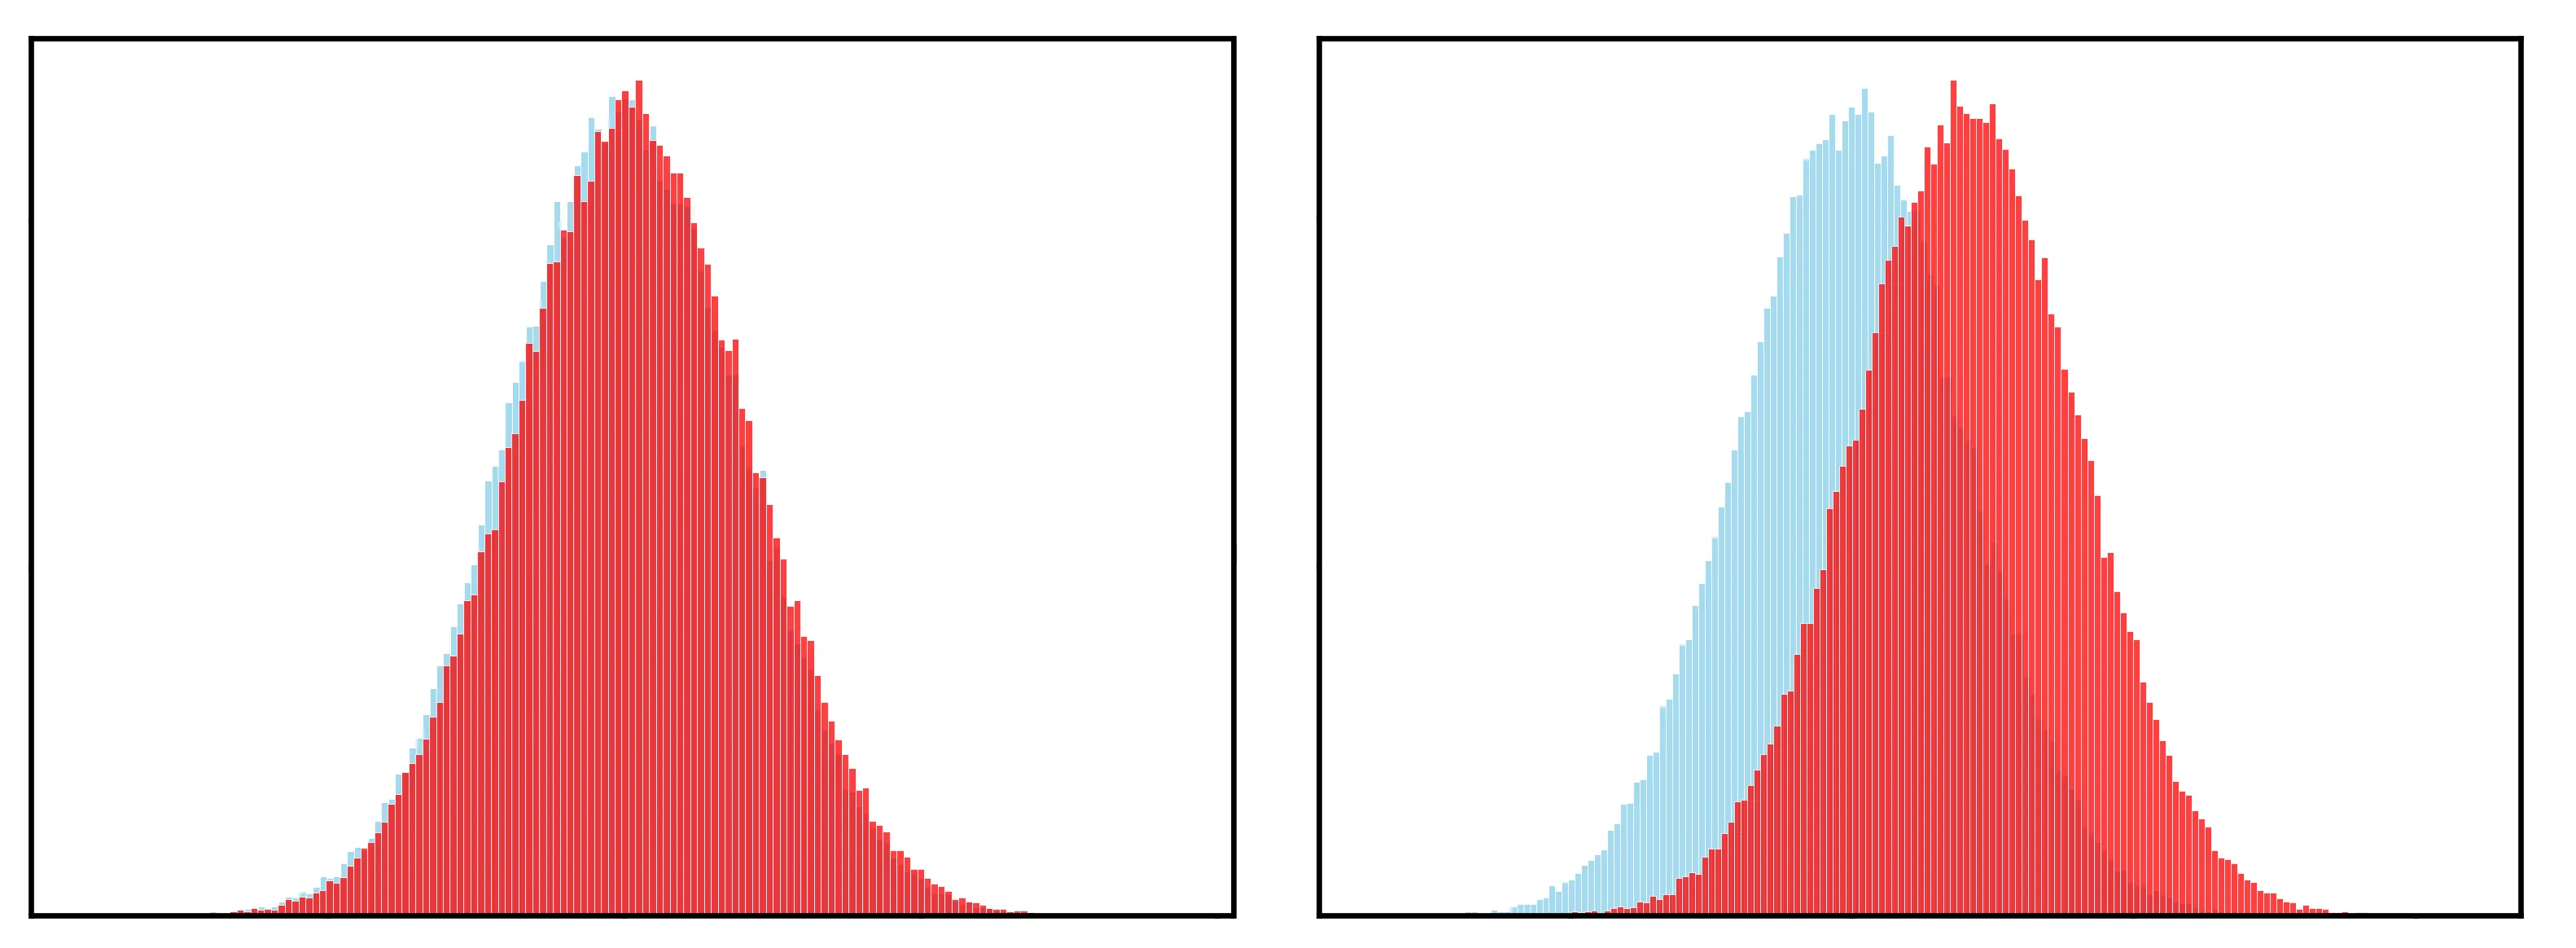
\includegraphics[width=\textwidth]{img/colmogorov-smirnov.png}
    \captionof{figure}{Kolmogorov-Smirnov visualisation}
\end{center}

Мой анализ здесь и далее был основан на том, что, зафиксировав начальные параметры в системе, порождающей ряд Лоренца $(10,28,8/3)$, я генерировал ряды, в которых один или несколько значений отличались на 1-2\% от оригинальных (из-за чувствительности ряда Лоренца к начальным параметрам порождаемые временные ряды сильно отличались от изначального), а затем анализировал «ближайшие» (по метрике) ряды и добавлял данные для обучения в оригинальный ряд для повышения точности предсказания.

\begin{center}
    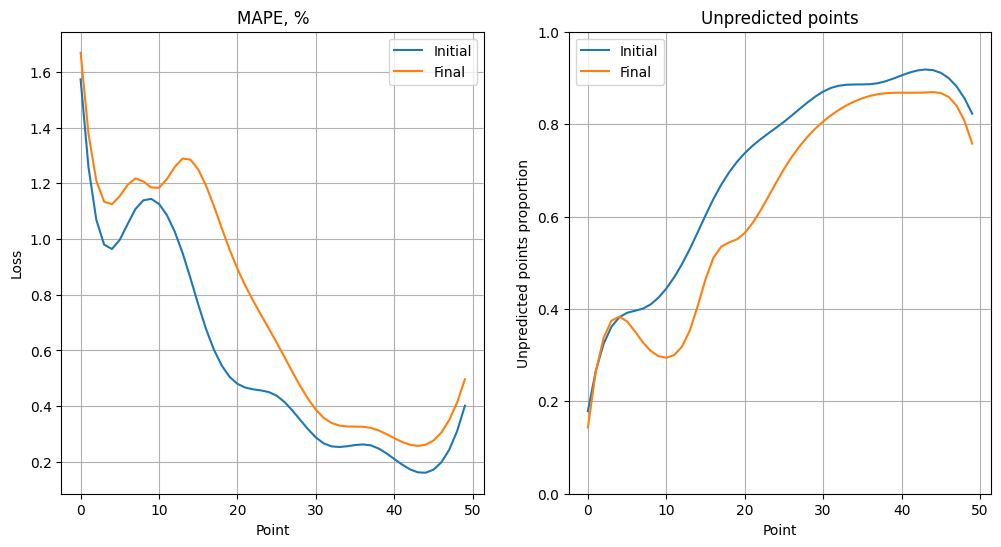
\includegraphics[width=\textwidth]{img/colmogorov.png}
    \captionof{figure}{Original series (train=1000) | Colmogorov mixing (train=5000)}
\end{center}

Таким образом, удалось уменьшить число непрогнозируемых точек при небольшом увеличении ошибки, а значит, этот метод в целом применим в проверке на то, что ряд "подходит" для добавления данных из него.

\subsection{Dynamic Time Warping}

Метод DTW (Dynamic Time Warping) сравнивает временные ряды напрямую, но, в отличие от, к примеру, стандартного евклидова расстояния, он учитывает временные искажения при сравнении рядов (растяжение / сжатие, см. рис.) и теоретически может дать более точную оценку "похожести" рядов.

\begin{center}
    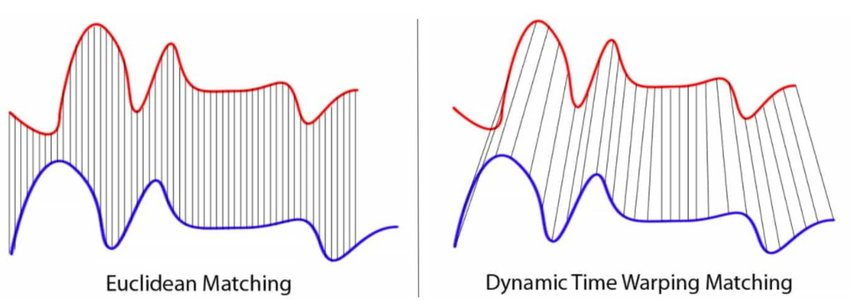
\includegraphics[width=\textwidth]{img/dtw_vis.png}
    \captionof{figure}{DTW visualisation}
\end{center}

В процессе анализа я подбирал ряды из ближайших к оригинальному для улучшения метрики. После более чем 15 операций добавления данных из других рядов к изначальному, были получены следующие результаты:

\begin{center}
    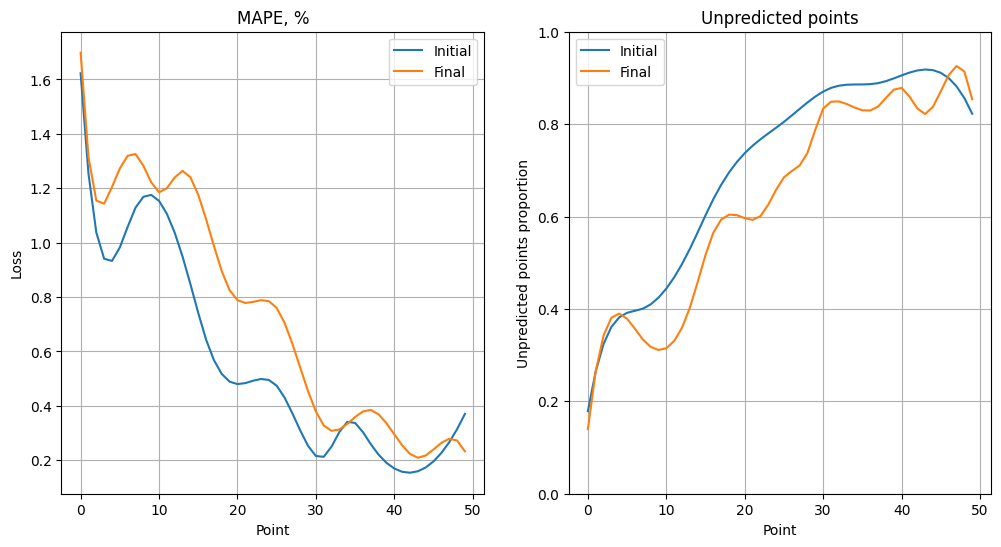
\includegraphics[width=\textwidth]{img/dtw.png}
    \captionof{figure}{Original series (train=1000) | DTW mixing (train=5000)}
\end{center}

Можно заметить, что для этого метода результаты даже немного хуже, чем для критерия Колмогорова-Смирнова, хотя теоретически этот метод более точный. Я могу объяснить этот факт тем, что у ряда Лоренца сложная структура, которая, по-видимому, не может быть точно проанализирована методом DTW, и обычное евклидово расстояние оказывается более репрезентативной метрикой

\subsection{Анализ ординальных структур}

Некоторые методы сравнивают не временные ряды напрямую, а преобразовывают их в иные структуры и сводят анализ рядов к анализу этих структур. Одними из более распространённых являются ординальные структуры. Сам переход от ряда заключается в том, что каждый мотив заменяется перестановкой, которая, при её применении к данному мотиву, сортирует его элементы (к примеру, $(0.1,0,0.2)\rightarrow (1,0,2)$). Далее формируется вектор $p\in\mathbb{R}^{(L+1)!}$, где $i-$ая координата – доля $i-$ой перестановки среди всех. Такие вероятностные векторы и анализируются вместо самих временных рядов.

Изначально у меня было 2 принципиально разных подхода для сравнения вероятностных векторов. Во-первых, обычная норма, то есть $\|p_1-p_2\|_F$. Во-вторых, более продвинутый подход, использующий энтропию векторов как рядов: $H\left(\frac{p_1+p_2}{2}\right)-\frac{1}{2}H(p_1)-\frac{1}{2}H(p_2)$. Однако, после проведения сравнительного анализа этих двух подходов оказалось, что позиции каждого из 125 сгенерированных рядов Лоренца при сортировке по каждой из приведённых метрик сильно скоррелированы (см. рис.).

\begin{center}
    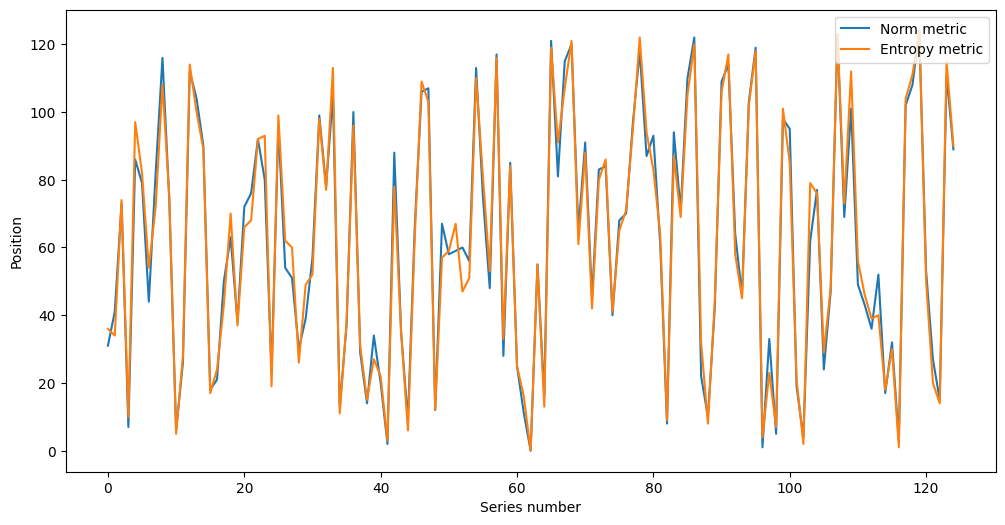
\includegraphics[width=\textwidth]{img/metrics.png}
    \captionof{figure}{Different metrics based on probability vectors comparison}
\end{center}

Таким образом, я принял решение рассматривать эти два подхода вместе, учитывая каждый из них с весом 0.5. Далее, мною были проведены более 15 операций добавления данных из ближайших к оригинальному, и были получены следующие результаты:

\begin{center}
    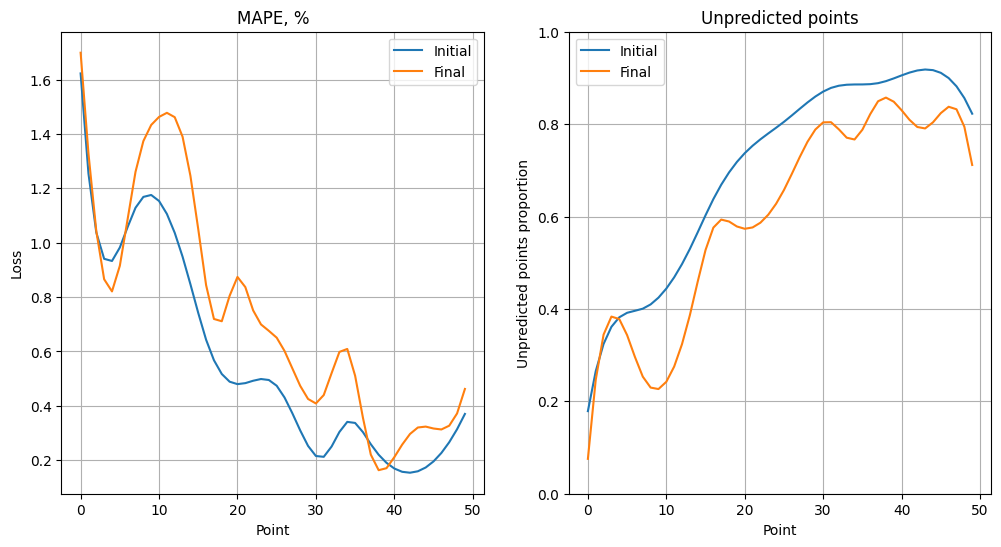
\includegraphics[width=\textwidth]{img/ord_str.png}
    \captionof{figure}{Original series (train=1000) | Ordinal Structures mixing (train=5000)}
\end{center}

Можно заметить, что ошибка в данном случае выросла сильнее, но число непрогнозируемых точек заметно уменьшилось в сравнении с прошлым методом, что особенно видно в конце, когда по экспоненциальному закону ошибки график должен стремиться к $1$ (большинство точек непрогнозируемые), однако тот лишь слегка превышает $0.8$.

\section{Анализ реального временного ряда}

В качестве реального ряда для оценки полученных методов было решено использовать временные ряды потребления электроэнергии в разных странах. Для того, чтобы нелинейная динамика давала прирост качества, необходимо, чтобы ряды были не только были примерно похожи, но и чтобы они имели структуру, похожую на ряды Лоренца. Данное свойство позволило бы успешнее перенести результаты исследования для ряда Лоренца на реальный ряд. Таким образом, идеальным решением стал ряд потребления электроэнергии, в котором промежуток между соседними точками составляет 1 час. Такие ряды, как нетрудно понять, имеют амплитуду, обусловленную пониженным потреблением ночью и повышенным потреблением днём. Ниже приведены части временных рядов для 20 европейских стран. Использование нормализации обусловлено тем, что в разных странах в силу различных факторов разные значения потребления, так что для анализа необходимо было ограничить все ряды отрезком $[0,1]$.

\begin{center}
    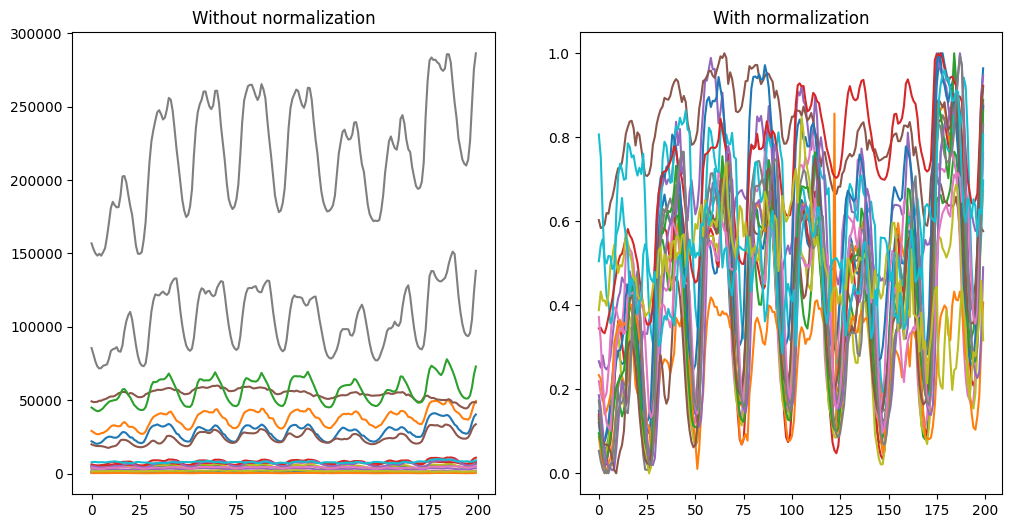
\includegraphics[width=\textwidth]{img/consumption_series.png}
    \captionof{figure}{Electricity consumption in Europe in 2024}
\end{center}

Далее я применил метод, который лучше всех показал себя при прогнозировании ряда Лоренца - анализ ординальных структур. В результате анализа 10 добавлений данных из близких по метрике рядов были получены следующие результаты. 

\begin{center}
    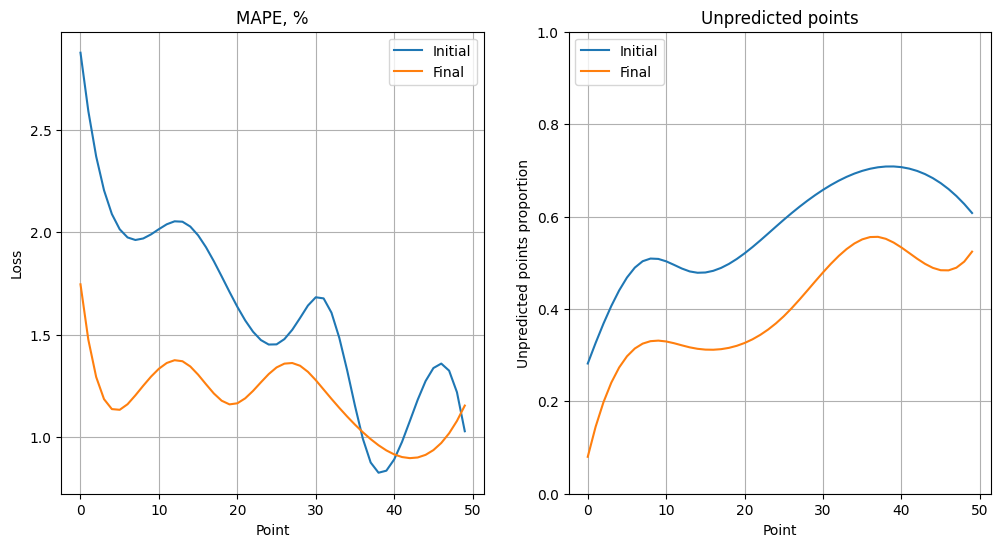
\includegraphics[width=\textwidth]{img/consumption.png}
    \captionof{figure}{Original series (train=1000) | Ordinal Structures mixing (train=5000)}
\end{center}

Таким образом, добавление других рядов положительно сказалось как на количестве непрогнозируемых точек, так и на ошибке. А значит данный метод вполне применим не только на синтетических рядах таких, как ряд Лоренца, но и на реальных данных, которые меньше поддвержены математическим законам и являются, по большей части, хаотическими.

\section{Заключение}

Итак, в результате работы над данным проектом я сделал следующие выводы

\begin{enumerate}
    \item Применение методов нелинейной динамики значительно улучшило качество прогнозирования многомерных хаотических временных рядов. Использование данных, полученных из других временных рядов, привело к увеличению обучающей выборки и, как следствие, повышению точности прогнозов при фиксированной максимальной допустимой ошибке.
    
    \item Рассмотренные методы - критерий Колмогорова-Смирнова, Dynamic Time Warping, анализ ординальных структур - продемонстрировали эффективность при прогнозировании. В то время как метод DTW теоретически должен был показать лучшее качество в сравнении с критерием Смирнова, поскольку учитывает растяжение и сжатие рядов, последний оказался более успешным при прогнозировании. В то же время анализ ординальных структур существенно повысил качество прогнозов, если сравнивать с упомянутыми выше методами, что особенно важно при предсказаниях на много шагов вперёд.
    
    \item Исследование продемонстрировало, что результаты, полученные на синтетическом ряде Лоренца, могут быть успешно экстраполированы на реальные ряды такие, как данные о потреблении электроэнергии. Наличие сложных структурных особенностей, характерных как для реальных, так и для синтетических рядов, подтверждает потенциал методов нелинейной динамики для их применения на практике.
    
    \item Теоретические выводы говорят о том, что увеличение объёма обучающей выборки может привести к более точным и стабильным прогнозам. Так что дальнейшее исследование может быть направлено на оптимизацию различных алгоритмов прогнозирования и разработку новых методов, которые бы объединяли преимущества разных подходов для решения задач прогнозирования хаотических систем с целью возможности расширения обучающей выборки
\end{enumerate}

Таким образом, проделанная работа доказывает, что методы нелинейной динамики являются мощным инструментом для прогнозирования многомерных хаотических временных рядов, а также имеют большой потенциал для практического применения в различных областях, в которых требуются стабильно точные прогнозы.

\newpage
\bibliographystyle{plainurl}
\bibliography{bibl}

\end{document}